% Define the page style
\fancypagestyle{chapterstyle}{
   \fancyhead[L]{\nouppercase{\rightmark}}
   \fancyhead[R]{Projet de fin d'etudes 2023-2024}
   \fancyfoot[C]{\vspace{20pt}\thepage} % Adjust the vertical space here
   \setlength{\headheight}{20pt}
   \setlength{\footskip}{30pt} % Adjust the value as needed
}


\chapter{Analyse et Spécifications des besoins}
\pagestyle{chapterstyle}
Dans ce chapitre, nous menons une étude approfondie du processus existant en mettant
en évidence les solutions de gestion de recrutement actuellement adoptées par 4D, ainsi
que les plateformes et les outils qui existent déjà sur le marché. Cela est dans l’objectif
de cerner les besoins fonctionnels et techniques auxquels doit répondre le projet.

\newpage
\vspace{1cm}

%-------------Spécifications des exigences-----------

\section{Analyse de l'existant}
Actuellement, chez 4D, il n’existe pas de plateforme centralisée pour gérer le processus
de recrutement. Les recruteurs utilisent plusieurs outils qui varient selon les différentes
étapes du processus, incluant LinkedIn, Gmail entre autres. Cette diversification des outils
entraîne plusieurs problèmes tels que le risque de perte d’informations, des difficultés de
coordination, ainsi qu’un temps de traitement des candidatures plus élevé. Ce processus
passe en fait par plusieurs étapes, notamment :

\begin{enumerate}
   \item[ • ] \textbf{Publication des annonces :} le processus de recrutement débute par la publication des offres d’emploi sur LinkedIn. Les recruteurs de 4D rédigent des annonces
   détaillées incluant les qualifications requises, les responsabilités du poste, ainsi que
   les informations sur l’entreprise. Ces annonces contiennent une adresse e-mail dédiée
   où les candidats peuvent envoyer leurs candidatures..
   \item[ • ] \textbf{Réception des candidatures :} Les candidats intéressés par les postes publiés
   envoient leur dossier de candidature par e-mail à l’adresse fournie dans l’annonce. Ce
   dossier comprend généralement un CV et une lettre de motivation. Les candidatures
   sont ensuite centralisées dans une boîte de réception gérée par les recruteurs.
   
   \item[ • ] \textbf{Traitement manuel des candidatures :} Les recruteurs examinent manuellement
   chaque candidature reçue. Ils évaluent les CV et les lettres de motivation pour
   déterminer si les candidats répondent aux critères du poste. Cette phase implique
   une analyse approfondie des compétences et de l’expérience des candidats et peut
   être sujette à des risques d’erreurs humaines, d’oublis ou de retards.
   
   \item[ • ] \textbf{Planification des entretiens :} Une fois les candidatures présélectionnées, les recruteurs contactent les candidats par e-mail pour organiser des entretiens oraux
   sans qu’il y ait des tests techniques écrits pour mieux évaluer les compétences des
   candidats. À ce stade, ils utilisent l’application Calendly. Il s’agit d’un outil de planification en ligne qui permet de synchroniser les agendas des recruteurs avec les
   disponibilités des candidats. Les recruteurs envoient un lien Calendly aux candidats,
   leur permettant de choisir un créneau horaire parmi ceux disponibles.
   \item[ • ] \textbf{Programmation des réunions :} Après que les candidats ont sélectionné leur
   horaire de disponibilité via Calendly, les recruteurs programment les entretiens de
   façon manuelle sur Zoom. Ils créent une réunion pour chaque entretien prévu et
   envoient le lien de la réunion aux candidats.
   \item[ • ] \textbf{Réalisation des entretiens :}  Les entretiens se déroulent à la date et à l’heure
   convenues, via Zoom. Les candidats, qui sont sélectionnés, sont informés par e-mail
   afin qu’ils entament le processus d’intégration.
   
\end{enumerate}

En bref, le processus de recrutement actuel chez 4D repose sur une série d’étapes qui
nécessitent beaucoup d’interventions humaines. De ce fait, il pourrait avoir des améliorations et bénéficier d’une digitalisation plus automatisée et intégrée. Le diagramme BPMN
suivant résume l’ensemble des étapes du processus :

\begin{figure}[h]
   \centering
   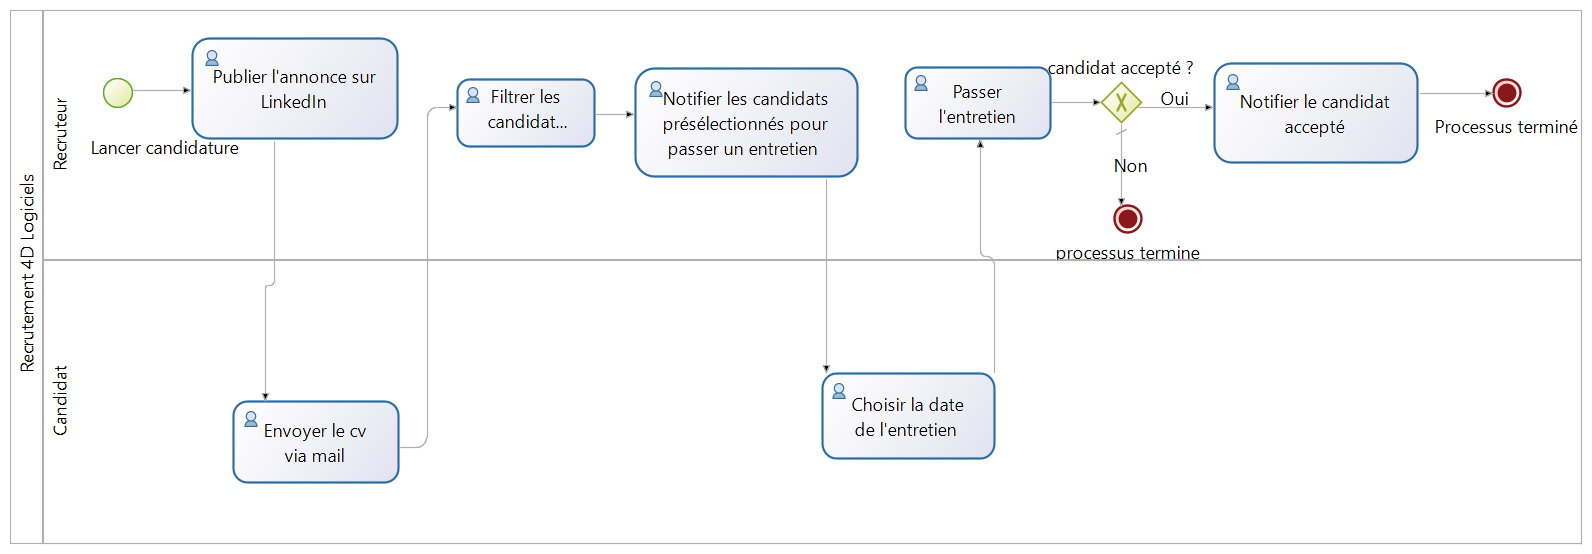
\includegraphics[scale=0.3]{Images/BPMN1.png} 
   \caption{Diagramme BPMN du processus actuel de recrutement chez 4D}
   \label{fig:BPMN1}
\end{figure}




%--------- Etat de l'art ----------

\section{Benchmarking des principales solutions de recrutement}
Il existe une multitude de plateformes qui sont destinées à la gestion de recrutement
et qui proposent une variété de fonctionnalités qui facilitent ce processus. Parmi ces plateformes, nous citons :

% \subsection{Solutions existantes sur le marché}
% \subsubsection{Indeed}
% Indeed est l’une des plateformes de recherche d’emploi les plus populaires au monde,
% fondée en 2004. Les employeurs peuvent publier des offres d’emploi directement sur la
% plateforme, en spécifiant les détails du poste, les qualifications requises et les avantages
% offerts. Ces publications peuvent être sponsorisées, permettant aux offres d’emploi de gagner en visibilité et d’apparaître en haut des résultats de recherche. En plus, les recruteurs
% peuvent définir des questions de présélection pour filtrer les candidatures et accéder à des
% statistiques détaillées sur les performances de leurs offres d’emploi, y compris le nombre
% de vues et de candidatures reçues.\\
% \begin{figure}[h]
%    \centering
%    
\includegraphics[scale=0.6]{Images/indeed.png} % Replace with the actual filename of the IBM logo image
%    \caption{Logo de Indeed}
%    \label{fig:indeed}
% \end{figure}
% Malgré la notoriété du moteur de recherche d’offres d’emploi de Indeed, certains points
% freinent son bon fonctionnement. Un utilisateur a rapporté avoir reçu plusieurs messages
% du site, y compris des refus pour des offres auxquelles il n’avait pas postulé. Les responsables chez Indeed ont attribué ce problème à un piratage de compte, ce qui soulève des
% préoccupations de sécurité. Du côté des employeurs, certains expriment leur insatisfaction
% quant à la qualification des candidats reçus via la plateforme.\\
% De plus, Indeed est une plateforme largement utilisée par de nombreuses entreprises,
% ce qui rend la concurrence accrue pour attirer l’attention des candidats. Pour garantir
% une bonne visibilité des offres, il est souvent nécessaire de payer pour des annonces sponssorisées. De plus, Indeed n’intègre pas de calendrier ni d’outil de gestion des entretiens,
% obligeant les recruteurs à utiliser des outils externes pour ces tâches.\\


% \subsubsection{LinkedIn Recruiter}
% LinkedIn Recruiter est un outil de recrutement professionnel intégré à LinkedIn, le plus
% grand réseau professionnel en ligne. Il permet aux recruteurs de rechercher, de contacter
% et de gérer des candidats potentiels directement sur la plateforme. Les recruteurs peuvent
% utiliser des filtres détaillés pour affiner leur recherche de candidats, tels que les compétences, l’expérience, la localisation et l’éducation, tout en bénéficiant des suggestions des
% candidats de la plateforme. En outre, les recruteurs peuvent créer des projets pour organiser et suivre les candidats intéressants pour différents postes. LinkedIn facilite ainsi la
% communication, vu que les recruteurs peuvent envoyer des messages InMail directement
% aux candidats, même s’ils ne sont pas connectés sur LinkedIn.\\

% \begin{figure}[h]
%    \centering
%    
\includegraphics[scale=0.6]{Images/linkedin.png} % Replace with the actual filename of the IBM logo image
%    \caption{Logo de LinkedIn Recruiter}
%    \label{fig:LinkedIn}
% \end{figure}

% Bien que LinkedIn Recruiter offre une grande base de données de candidats, la visibilité des offres d’emploi peut être limitée sans une licence payante qui coute 170\$ par mois
% seulement pour une licence LinkedIn Recruiter Lite. Ainsi, le recrutement sur LinkedIn
% repose fortement sur la présence numérique et les compétences en réseautage d’un candidat. Ajoutons à cela que certains utilisateurs ont des paramètres de confidentialité stricts
% qui limitent leur visibilité sur LinkedIn.

% \subsubsection{Rekrute}
% Rekrute.ma est un site de recrutement en ligne populaire au Maroc, lancé en 2006.
% Il met en relation les chercheurs d’emploi avec les recruteurs de divers secteurs. Le site
% propose des annonces couvrant de nombreux secteurs, notamment la finance, l’ingénierie,
% le marketing, les ressources humaines et plus encore. Ainsi, Rekrute.ma offre des ressources pour aider les candidats dans leur recherche d’emploi, comme des conseils pour
% les entretiens, la rédaction de CV, etc.

% \begin{figure}[h]
%    \centering
%    
\includegraphics[scale=0.6]{Images/rekrute.png} % Replace with the actual filename of the IBM logo image
%    \caption{Logo de Rekrute}
%    \label{fig:rekrute}
% \end{figure}

% Cependant, la popularité du site entraîne une forte concurrence pour les offres d’emploi, ce qui peut rendre difficile pour certains candidats de se démarquer.

% \subsubsection{Odoo : Module de recrutement}

% Odoo est une suite d’applications de gestion d’entreprise open source qui couvre divers
% aspects des opérations d’une entreprise, y compris la gestion des ressources humaines. Le
% module de recrutement d’Odoo est conçu pour aider les entreprises à gérer leurs processus de recrutement, de la publication des offres d’emploi à l’intégration des nouveaux
% employés. En effet, les entreprises peuvent créer et publier des offres d’emploi directement sur leur site web ou sur des portails d’emploi intégrés. De plus, avec un système de
% suivi des candidatures (Applicant Tracking System), les recruteurs peuvent suivre chaque
% étape du processus de recrutement, de la réception de la candidature à l’entretien et à
% l’embauche.\\
% Ce module peut être intégré avec d’autres modules Odoo, comme la gestion des ressources humaines, les feuilles de temps et la gestion des projets, ce qui permet une gestion
% globale des employés.

% \begin{figure}[h]
%    \centering
%    
\includegraphics[scale=0.6]{Images/odoo.png} % Replace with the actual filename of the IBM logo image
%    \caption{Logo de Odoo}
%    \label{fig:odoo}
% \end{figure}

% Néanmoins, de nombreuses limitations peuvent freiner l’adoption de ce module. L’installation et la configuration initiales nécessitent une expertise technique, surtout pour les
% personnalisations avancées. En outre, certaines fonctionnalités, telles que les tests, ne sont
% pas disponibles par défaut et nécessitent des modules additionnels ou des personnalisations, ce qui augmente le cout et le temps de traitement.\\
% Selon cette étude générale de diverses plateformes de recrutement, il apparaît que
% les fonctionnalités avancées proposées par celles-ci sont souvent coûteuses et visent à
% répondre aux besoins d’un large éventail d’entreprises. Ce qui entraîne une augmentation
% de la concurrence qui nécessite fréquemment le passage à un plan payant. Ajoutons à
% cela que pour répondre de manière optimale à ses besoins spécifiques, 4D nécessite une
% plateforme de recrutement interne, développée avec ses propres technologies et alignée
% avec ses exigences et processus internes.




\subsection{Solutions existantes sur le marché}


% \begin{longtable}{|p{2cm}|p{4.5cm}|p{4cm}|p{4cm}|}
%    \caption{Comparaison des solutions de recrutement} \\
%    \hline
%    \rowcolor{gray!30}
%    \textbf{Solution} & \textbf{Fonctionnalités principales} & \textbf{Avantages} & \textbf{Inconvénients} \\
%    \hline
%    \small Indeed & 
%    \small - Publication d'offres d'emploi \newline
%    - Recherche de CV \newline
%    - Campagnes sponsorisées &
%    \small - Grande popularité \newline
%    - Facilité d'utilisation &
%    \small - Qualité variable des candidats \newline
%    - Options limitées sans paiement \\
%    \hline
%    \small LinkedIn Recruiter & 
%    \small - Recherche avancée de candidats \newline
%    - Gestion des talents \newline
%    - Analyses et rapports &
%    \small - Large base de données de candidats \newline
%    - Outils de sourcing puissants &
%    \small - Coût élevé \newline
%    - Complexité d'utilisation pour les débutants \\
%    \hline
%    \small Rekrute & 
%    \small - Publication d'offres d'emploi \newline
%    - Base de données de CV \newline
%    - Solutions RH intégrées &
%    \small - Forte présence en Afrique du Nord \newline
%    - Interface adaptée aux marchés locaux &
%    \small - Moins connu en dehors des marchés ciblés \newline
%    - Options limitées pour les entreprises internationales \\
%    \hline
%    \small Odoo: Module de recrutement & 
%    \small - Suivi des candidatures \newline
%    - Intégration avec autres modules Odoo \newline
%    - Personnalisation des processus de recrutement &
%    \small - Intégration complète avec l'écosystème Odoo \newline
%    - Grande flexibilité et personnalisation &
%    \small - Complexité de configuration initiale \newline
%    - Nécessite des compétences techniques pour la personnalisation \\
%    \hline
% \end{longtable}



{\small % Début de la taille de police small
\renewcommand{\arraystretch}{1.5}
\begin{longtable}{|p{2cm}|p{4.5cm}|p{4cm}|p{4.2cm}|}
\caption{Comparaison des solutions de recrutement} \\
\hline
\rowcolor{gray!30}
\textbf{Solution} & \textbf{Fonctionnalités principales} & \textbf{Avantages} & \textbf{Inconvénients} \\
\hline
\textbf{Indeed} & 
\begin{minipage}[t]{5cm}
- Publication d'offres \\ 
d'emploi \\
- Recherche de CV \\
- Campagnes sponsorisées\\
\end{minipage} &
\begin{minipage}[t]{5cm}
- Grande popularité \\
- Facilité d'utilisation
\end{minipage} &
\begin{minipage}[t]{5cm}
- Qualité variable\\
 des candidats \\
- Options limitées sans\\ 
paiement
\end{minipage} \\
\hline
\textbf{LinkedIn Recruiter} & 
\begin{minipage}[t]{5cm}
- Recherche avancée \\ 
de candidats \\
- Gestion des talents \\
- Analyses et rapports\\
\end{minipage} &
\begin{minipage}[t]{5cm}
- Large base de \\
données de candidats \\
- Outils de sourcing \\ 
puissants
\end{minipage} &
\begin{minipage}[t]{5cm}
- Coût élevé \\
- Complexité d'utilisation\\ 
pour les débutants
\end{minipage} \\
\hline
\textbf{Rekrute} & 
\begin{minipage}[t]{5cm}
- Publication d'offres \\ 
d'emploi \\
- Base de données de CV \\
- Solutions RH intégrées
\end{minipage} &
\begin{minipage}[t]{5cm}
- Forte présence en \\
Afrique du Nord \\
- Interface adaptée\\ 
aux marchés locaux
\end{minipage} &
\begin{minipage}[t]{5cm}
- Moins connu en dehors \\ 
des marchés ciblés \\
- Options limitées pour les \\
entreprises internationales\\

\end{minipage} \\
\hline
\textbf{Odoo:  Module de recrutement} & 
\begin{minipage}[t]{5cm}
- Suivi des candidatures \\
- Intégration avec autres \\ 
modules Odoo \\
- Personnalisation des \\
processus de recrutement
\end{minipage} &
\begin{minipage}[t]{5cm}
- Intégration complète\\ 
avec l'écosystème Odoo \\
- Grande flexibilité \\ 
et personnalisation
\end{minipage} &
\begin{minipage}[t]{5cm}
- Complexité de \\ 
configuration initiale \\
- Nécessite des \\ 
compétences techniques \\ 
pour la personnalisation\\
\end{minipage} \\
\hline
\end{longtable}
} % Fin de la taille de police small


\subsection{Synthèse de l’étude benchmarking}
Cette étude comparative nous a conduits à remarquer clairement 
l'insuffisance des différentes solutions de recrutement disponibles 
sur le marché. Certaines répondent aux besoins fonctionnels liés 
seulement aux modules administratifs, et d’autres présentent des 
complexités liées au déploiement et à l’installation. De plus, 
la plupart des solutions sont fermées à l’introduction de nouvelles 
fonctionnalités, révélant une absence totale de l’aspect évolutif des 
systèmes. D'où l’intérêt de penser à une solution moderne avec un aspect 
modulaire, évolutif, et en responsive design.

\subsection{Justification pour la Création d'une Plateforme de Recrutement chez 4D}
Avec ces observations en tête, il est crucial de développer une plateforme 
de recrutement interne chez 4D avec les éléments suivants :

\begin{itemize}
   \item[ • ] First item
   \item[ • ] Second item
   \item[ • ] Third item
\end{itemize}